% IEEE Conference Paper Template
% Resampling and Model Selection on UCI Auto MPG Dataset

\documentclass[conference]{IEEEtran}
\usepackage{cite}
\usepackage{amsmath,amssymb,amsfonts}
\usepackage{algorithmic}
\usepackage{graphicx}
\usepackage{textcomp}
\usepackage{xcolor}
\usepackage{booktabs}
\usepackage{multirow}
\usepackage{hyperref}
\usepackage[compatibility=false]{caption}
\usepackage{subcaption}
\usepackage{array}
\usepackage{float}

\begin{document}

\title{Resampling and Model Selection Methods for Fuel Efficiency Prediction: An Application to the UCI Auto MPG Dataset}

\author{
\IEEEauthorblockN{Riyad Abdurahimov, Gabil Gurbanov}
\IEEEauthorblockA{Applied Machine Learning, Course Project 3\\
\url{https://github.com/ggurbanov12098/AppliedML-P3}\\
Instructor: Dr. Samir Rustamov}
}

\maketitle

\begin{abstract}
Predicting vehicle fuel efficiency from specifications is a fundamental regression problem in applied machine learning. This paper presents a comprehensive study of resampling and model selection methods on the University of California, Irvine (UCI) Auto Miles Per Gallon (MPG) dataset. We apply Cross-Validation (CV) (K=5, K=10, Leave-One-Out CV (LOOCV)), bootstrap resampling, subset selection (best subset, forward and backward stepwise), shrinkage methods (Ridge and Lasso regression), Principal Component Analysis (PCA), and Partial Least Squares (PLS). Polynomial regression on the weight feature is evaluated across degrees 1--8; all resampling methods consistently identify degree 2 as optimal. Subset selection with 10-fold CV selects four predictors (displacement, weight, model\_year, origin), achieving CV Root Mean Squared Error (RMSE) of 3.369 and R\textsuperscript{2} of 0.8113. Ridge and Lasso regressions yield optimal regularization parameter $\lambda \approx 0.001$ for both. PLS attains full Ordinary Least Squares (OLS) performance with fewer components than Principal Component Regression (PCR) due to its supervised formulation. The best overall model is OLS with the optimal 4-feature subset. An interactive Streamlit application demonstrates all methods and enables live MPG prediction.
\end{abstract}

\begin{IEEEkeywords}
Cross-validation, bootstrap, subset selection, Ridge regression, Lasso regression, principal component analysis, partial least squares, fuel efficiency, Auto MPG.
\end{IEEEkeywords}

%==============================================================================
\section{Introduction}
\label{sec:intro}
%==============================================================================

Predicting vehicle fuel efficiency (MPG) from engineering specifications is a classic regression task with practical relevance for automotive design and policy. The UCI Machine Learning Repository's Auto MPG dataset provides a well-studied benchmark for evaluating resampling and model selection techniques.

\subsection{Motivation}
Model complexity and predictor selection directly affect generalization performance. Overly complex models risk overfitting; overly simple models underfit. Resampling methods such as CV and bootstrap provide unbiased estimates of test error. Subset selection and shrinkage methods reduce dimensionality and improve interpretability. This work systematically compares these approaches on the Auto MPG dataset.

\subsection{Contributions}
\begin{itemize}
    \item Application of K-fold CV (K=5, K=10), LOOCV, and bootstrap to polynomial regression.
    \item Exhaustive subset selection with multiple criteria: Mallow's $C_p$, AIC, BIC, adjusted $R^2$, and CV MSE.
    \item Ridge and Lasso regression with bias--variance tradeoff analysis.
    \item PCA and PLS for dimensionality reduction, with comparison to OLS.
    \item An interactive Streamlit dashboard for exploration and live prediction.
\end{itemize}

\subsection{Paper Organization}
Section~\ref{sec:data} describes the dataset and preprocessing. Section~\ref{sec:method} outlines the methodology. Section~\ref{sec:experiments} details the experimental setup. Section~\ref{sec:results} presents results and discussion. Section~\ref{sec:conclusion} concludes.

%==============================================================================
\section{Dataset and Preprocessing}
\label{sec:data}
%==============================================================================

\subsection{Dataset}
The Auto MPG dataset contains 398 vehicles with 9 attributes. After removing 6 rows with missing \texttt{horsepower} and the non-numeric \texttt{car\_name} column, we obtain 392 samples and 7 predictors plus the target MPG. Table~\ref{tab:features} lists all variables.

\begin{table}[htbp]
\caption{Features and Target Variable}
\label{tab:features}
\begin{center}
\begin{tabular}{|l|l|}
\hline
\textbf{Variable} & \textbf{Description} \\
\hline
cylinders & Number of cylinders \\
displacement & Engine displacement (cubic inches) \\
horsepower & Engine horsepower \\
weight & Vehicle weight (lbs) \\
acceleration & Time 0--60 mph (seconds) \\
model\_year & Model year (mod 100, e.g., 70--82) \\
origin & Origin (1=USA, 2=Europe, 3=Japan) \\
\hline
\textbf{mpg} & \textbf{Target: Miles per gallon} \\
\hline
\end{tabular}
\end{center}
\end{table}

\subsection{Preprocessing}
Features are standardized (zero mean, unit variance) using \texttt{StandardScaler} before model selection and shrinkage methods. This ensures fair comparison across predictors with different scales.

\begin{figure}[htbp]
\centering
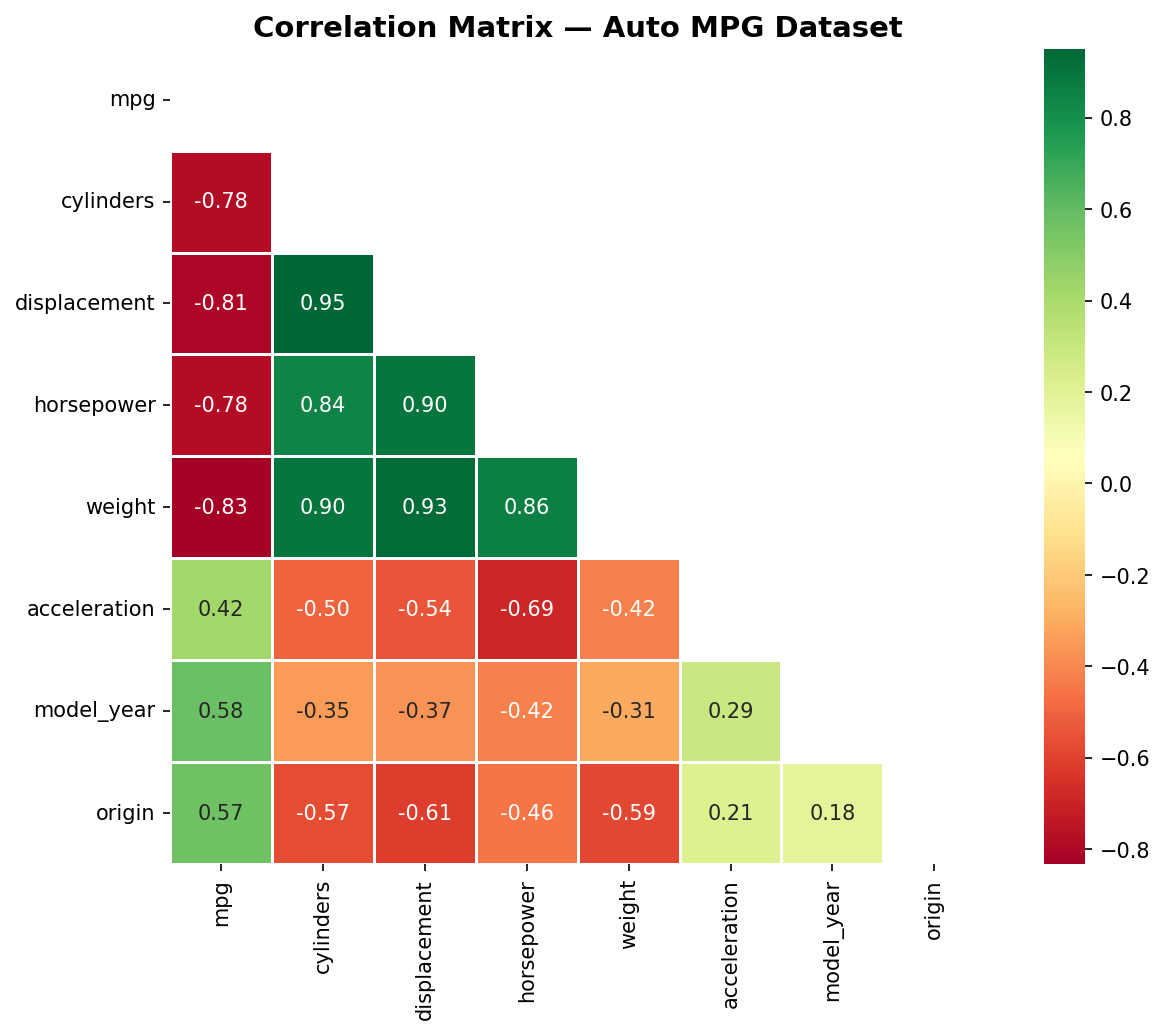
\includegraphics[width=\linewidth]{figures/correlation_heatmap.png}
\caption{Correlation matrix of features and target MPG. Weight has the strongest negative correlation with MPG.}
\label{fig:correlation}
\end{figure}

%==============================================================================
\section{Methodology}
\label{sec:method}
%==============================================================================

\subsection{Resampling Methods}
\label{sec:resampling}

\subsubsection{Cross-Validation}
CV partitions the data into $K$ folds. For each fold $k$, the model is trained on $K-1$ folds and evaluated on the $k$-th fold. The CV MSE is the average MSE over all folds:
\begin{equation}
\text{CV}(\lambda) = \frac{1}{K}\sum_{k=1}^{K} \text{MSE}_k(\lambda)
\end{equation}
We use K=5, K=10, and LOOCV (K=$n$).

\subsubsection{Bootstrap}
Bootstrap draws $B$ samples of size $n$ with replacement. Each bootstrap sample yields a training set; the OOB samples (not drawn) form the test set. The bootstrap MSE is:
\begin{equation}
\text{Boot}(\theta) = \frac{1}{B}\sum_{b=1}^{B} \text{MSE}_{\text{OOB},b}(\theta)
\end{equation}
We use $B=200$.

\subsubsection{Polynomial Regression}
For resampling, we fit polynomial regression of MPG on \textbf{weight} (highest correlation with MPG). The pipeline is: PolynomialFeatures $\rightarrow$ StandardScaler $\rightarrow$ LinearRegression. Degrees 1--8 are evaluated.

\subsection{Subset Selection}
\label{sec:subset}

\subsubsection{Best Subset}
For each $k \in \{1,\ldots,p\}$, we evaluate all $\binom{p}{k}$ subsets and select the one minimizing a criterion (e.g., MSE).

\subsubsection{Forward and Backward Stepwise}
Forward stepwise adds one predictor at a time by AIC. Backward stepwise removes one predictor at a time by AIC.

\subsubsection{Model Selection Criteria}
\begin{itemize}
    \item \textbf{Mallow's $C_p$:} $C_p = \frac{1}{n}(\text{RSS} + 2d\hat{\sigma}^2)$, where $d$ is the number of predictors.
    \item \textbf{AIC:} $\text{AIC} = n\log(\text{RSS}/n) + 2d$.
    \item \textbf{BIC:} $\text{BIC} = n\log(\text{RSS}/n) + d\log(n)$.
    \item \textbf{Adjusted $R^2$:} $R^2_{\text{adj}} = 1 - \frac{\text{RSS}/(n-d-1)}{\text{TSS}/(n-1)}$.
    \item \textbf{10-fold CV MSE:} Direct estimate of test error.
\end{itemize}

\subsection{Shrinkage Methods}
\label{sec:shrinkage}

\subsubsection{Ridge Regression (L2)}
Ridge minimizes
\begin{equation}
\sum_{i=1}^{n}(y_i - \mathbf{x}_i^\top\boldsymbol{\beta})^2 + \lambda \sum_{j=1}^{p}\beta_j^2
\end{equation}
The $\ell_2$ penalty shrinks all coefficients toward zero but does not set any to exactly zero.

\subsubsection{Lasso Regression (L1)}
Lasso minimizes
\begin{equation}
\sum_{i=1}^{n}(y_i - \mathbf{x}_i^\top\boldsymbol{\beta})^2 + \lambda \sum_{j=1}^{p}|\beta_j|
\end{equation}
The $\ell_1$ penalty can produce sparse solutions (exact zeros), performing implicit feature selection.

\subsubsection{Optimal \texorpdfstring{$\lambda$}{lambda}}
We select $\lambda$ via 10-fold CV using \texttt{RidgeCV} and \texttt{LassoCV}.

\subsection{PCA and PLS}
\label{sec:pca}

\subsubsection{Principal Component Analysis}
PCA finds orthogonal linear combinations of predictors that maximize variance. The first $M$ principal components capture the most variance. PCR regresses the target on these components.

\subsubsection{Partial Least Squares}
PLS finds latent components that maximize covariance with the target. Unlike PCA, PLS is supervised and thus uses MPG when constructing components.

\subsection{Evaluation Metric}
MSE and RMSE are used throughout:
\begin{equation}
\text{MSE} = \frac{1}{n}\sum_{i=1}^{n}(y_i - \hat{y}_i)^2, \quad \text{RMSE} = \sqrt{\text{MSE}}
\end{equation}

%==============================================================================
\section{Experimental Setup}
\label{sec:experiments}
%==============================================================================

\begin{itemize}
    \item \textbf{Resampling:} Polynomial degrees 1--8; K=5, K=10, LOOCV; OOB bootstrap with $B=200$; \texttt{random\_state=42}.
    \item \textbf{Subset selection:} Best subset, forward, backward; 10-fold CV for MSE.
    \item \textbf{Shrinkage:} $\lambda$ grid via \texttt{np.logspace}; 10-fold CV for Ridge and Lasso.
    \item \textbf{PCA/PLS:} 1--7 components; 10-fold CV for PCR and PLS MSE.
\end{itemize}

Implementation uses \texttt{scikit-learn}, \texttt{statsmodels}, and \texttt{pandas} in Python.

%==============================================================================
\section{Results and Discussion}
\label{sec:results}
%==============================================================================

\subsection{Resampling Methods}
\label{sec:resampling_results}

Table~\ref{tab:cv_mse} shows CV MSE by polynomial degree. All three CV methods (K=5, K=10, LOOCV) agree that \textbf{degree 2} is optimal. Bootstrap (Table~\ref{tab:bootstrap}) also selects degree 2. Higher degrees increase complexity without improving test error, indicating overfitting.

\begin{table}[htbp]
\caption{Cross-Validation MSE by Polynomial Degree}
\label{tab:cv_mse}
\begin{center}
\begin{tabular}{|c|c|c|c|}
\hline
\textbf{Degree} & \textbf{K=5} & \textbf{K=10} & \textbf{LOOCV} \\
\hline
1 & 18.93 & 18.84 & 18.85 \\
2 & \textbf{17.57} & \textbf{17.52} & \textbf{17.52} \\
3 & 17.61 & 17.57 & 17.58 \\
4 & 17.63 & 17.60 & 17.62 \\
5 & 17.69 & 17.61 & 17.63 \\
6 & 17.77 & 17.72 & 17.69 \\
7 & 17.77 & 17.75 & 17.67 \\
8 & 17.76 & 17.81 & 17.76 \\
\hline
\end{tabular}
\end{center}
\end{table}

\begin{table}[htbp]
\caption{Bootstrap MSE by Degree (B=200)}
\label{tab:bootstrap}
\begin{center}
\begin{tabular}{|c|c|c|}
\hline
\textbf{Degree} & \textbf{MSE} & \textbf{Std} \\
\hline
1 & 18.75 & 2.09 \\
2 & \textbf{17.45} & 2.13 \\
3 & 17.53 & 2.14 \\
4 & 17.60 & 2.14 \\
5 & 17.65 & 2.15 \\
6 & 17.77 & 2.10 \\
7 & 17.78 & 2.12 \\
8 & 18.00 & 2.24 \\
\hline
\end{tabular}
\end{center}
\end{table}

\begin{figure}[htbp]
\centering
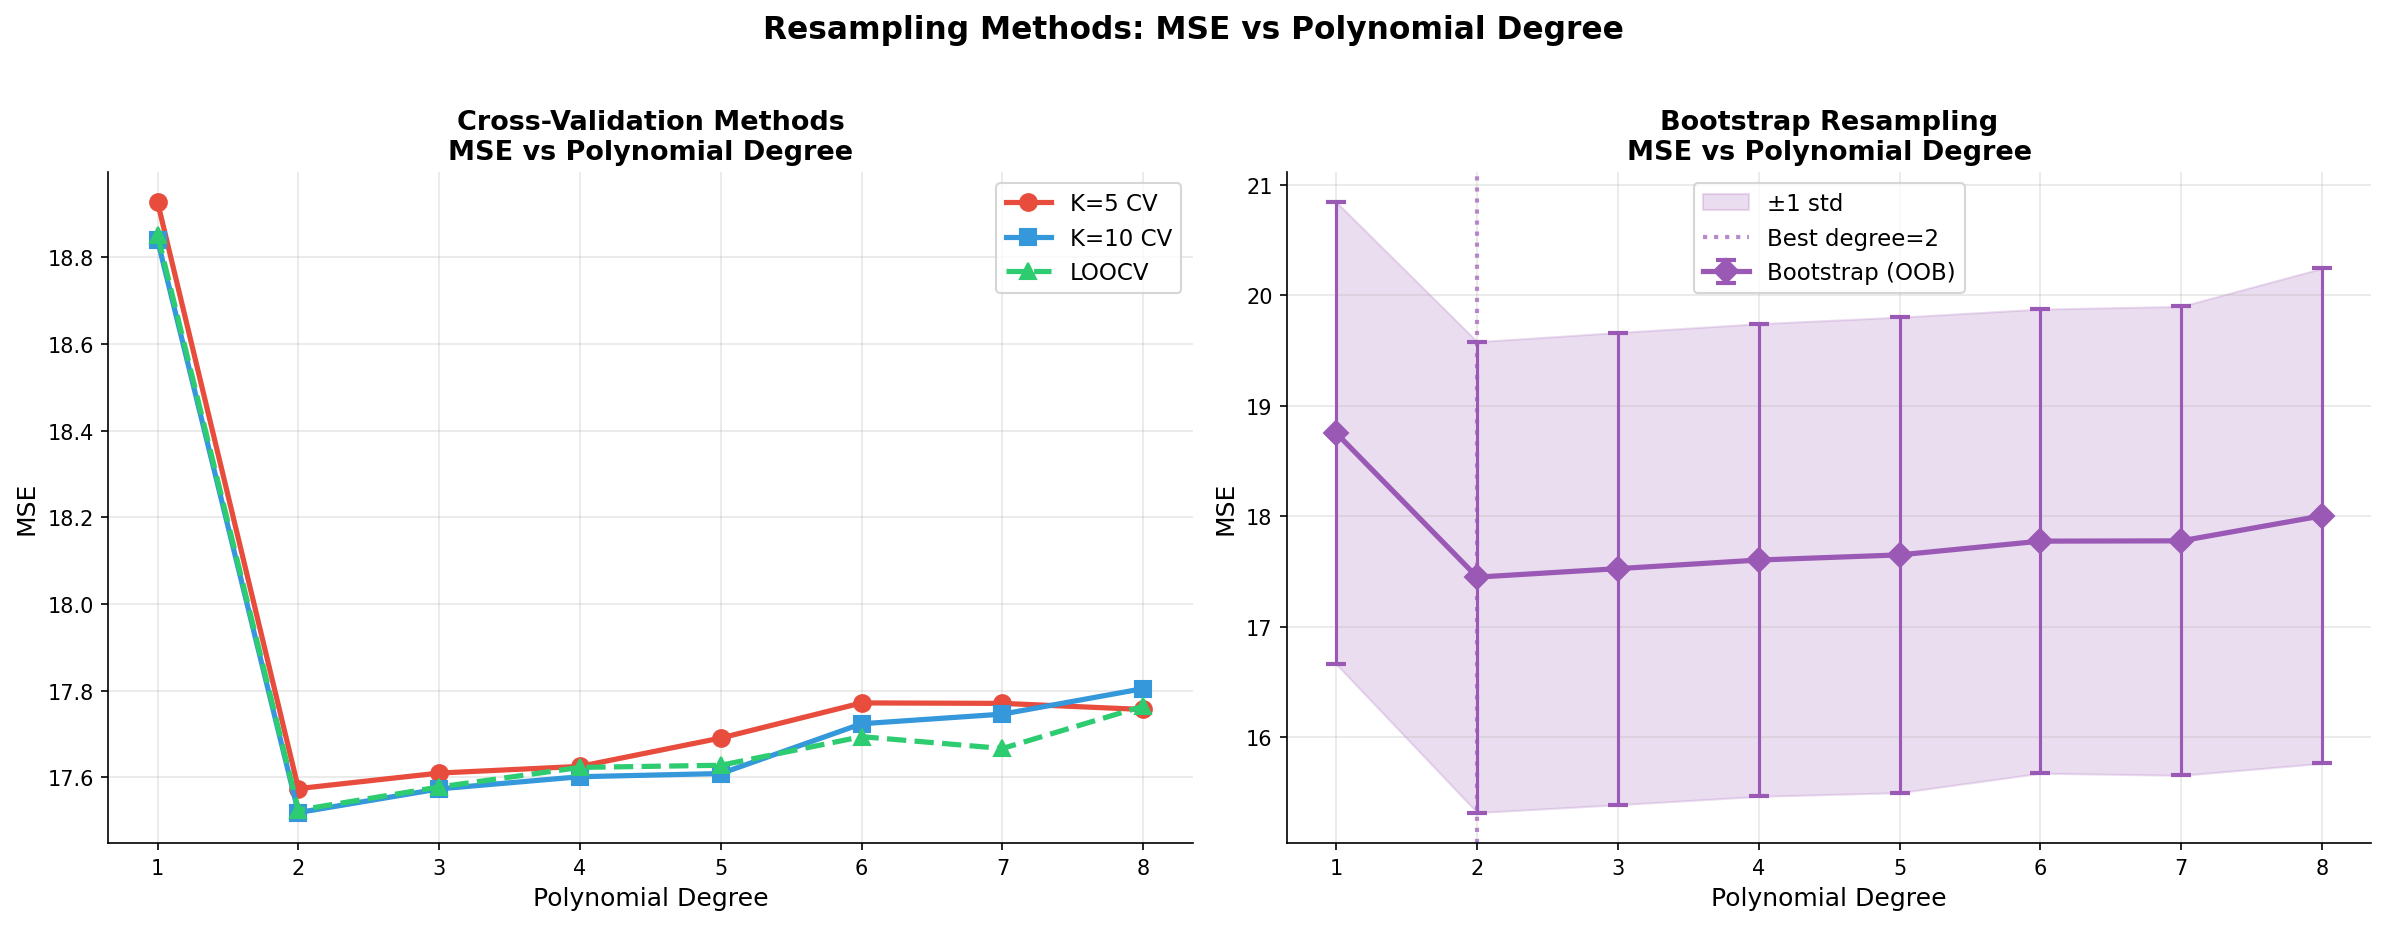
\includegraphics[width=\linewidth]{figures/resampling_comparison.png}
\caption{Resampling methods: (left) CV MSE vs polynomial degree for K=5, K=10, LOOCV; (right) Bootstrap MSE with $\pm$1 std error bars.}
\label{fig:resampling}
\end{figure}

\subsection{Subset Selection}
\label{sec:subset_results}

Table~\ref{tab:subset} summarizes best subset by number of predictors $k$. 10-fold CV MSE is minimized at \textbf{$k=4$} with predictors: displacement, weight, model\_year, origin. CV MSE = 11.353 vs 11.452 for full OLS, indicating slight improvement from removing redundant predictors.

\begin{table}[htbp]
\caption{Best Subset Selection: Metrics by Number of Predictors}
\label{tab:subset}
\begin{center}
\small
\begin{tabular}{|c|c|c|c|c|c|}
\hline
\textbf{$k$} & \textbf{AIC} & \textbf{BIC} & \textbf{$C_p$} & \textbf{Adj $R^2$} & \textbf{CV MSE} \\
\hline
1 & 2263.9 & 2271.9 & 18.73 & 0.692 & 18.84 \\
2 & 2081.1 & 2093.0 & 11.77 & 0.807 & 11.81 \\
3 & 2063.7 & 2079.6 & 11.26 & 0.816 & 11.38 \\
4 & 2064.3 & 2084.2 & 11.28 & 0.816 & \textbf{11.35} \\
5 & 2062.1 & 2086.0 & 11.22 & 0.818 & 11.40 \\
6 & 2061.6 & 2089.4 & 11.21 & 0.818 & 11.37 \\
7 & 2062.9 & 2094.7 & 11.24 & 0.818 & 11.45 \\
\hline
\end{tabular}
\end{center}
\end{table}

\begin{figure}[htbp]
\centering
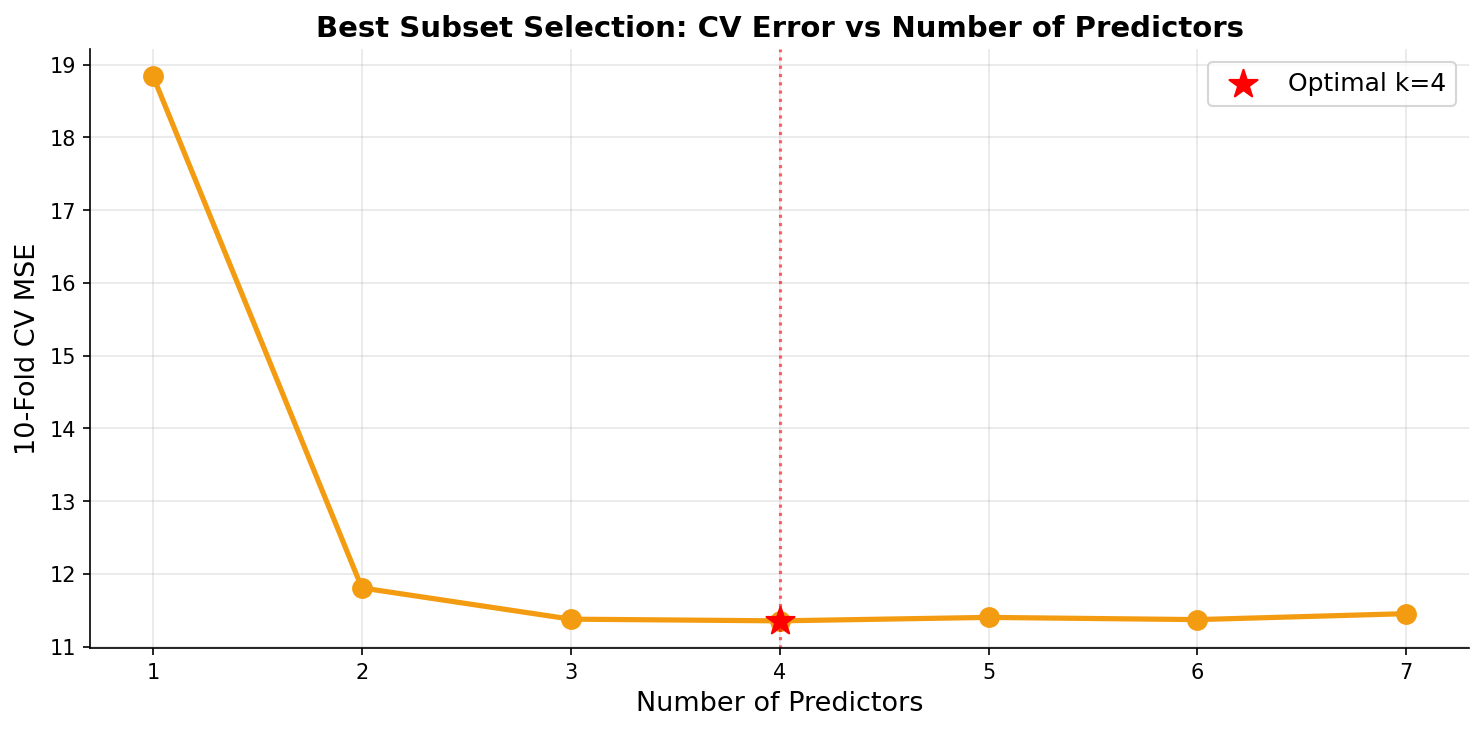
\includegraphics[width=\linewidth]{figures/subset_cv.png}
\caption{10-fold CV MSE vs number of predictors. Optimal $k=4$ (displacement, weight, model\_year, origin).}
\label{fig:subset_cv}
\end{figure}

\subsection{Shrinkage Methods}
\label{sec:shrinkage_results}

Both Ridge and Lasso yield \textbf{optimal $\lambda = 0.001$} via 10-fold CV. At this $\lambda$, coefficients are nearly identical to OLS (Table~\ref{tab:coefs}), indicating weak regularization is sufficient. The bias--variance tradeoff (Fig.~\ref{fig:bias_var}) shows that low $\lambda$ gives low test MSE; high $\lambda$ increases bias.

\begin{table}[htbp]
\caption{Coefficients at Optimal $\lambda$ (Ridge $=$ Lasso $=$ 0.001)}
\label{tab:coefs}
\begin{center}
\small
\begin{tabular}{|l|c|c|c|}
\hline
\textbf{Feature} & \textbf{OLS} & \textbf{Ridge} & \textbf{Lasso} \\
\hline
cylinders & $-0.84$ & $-0.84$ & $-0.82$ \\
displacement & 2.08 & 2.08 & 2.03 \\
horsepower & $-0.65$ & $-0.65$ & $-0.64$ \\
weight & $-5.49$ & $-5.49$ & $-5.48$ \\
acceleration & 0.22 & 0.22 & 0.22 \\
model\_year & 2.76 & 2.76 & 2.76 \\
origin & 1.15 & 1.15 & 1.14 \\
\hline
\end{tabular}
\end{center}
\end{table}

\begin{figure}[htbp]
\centering
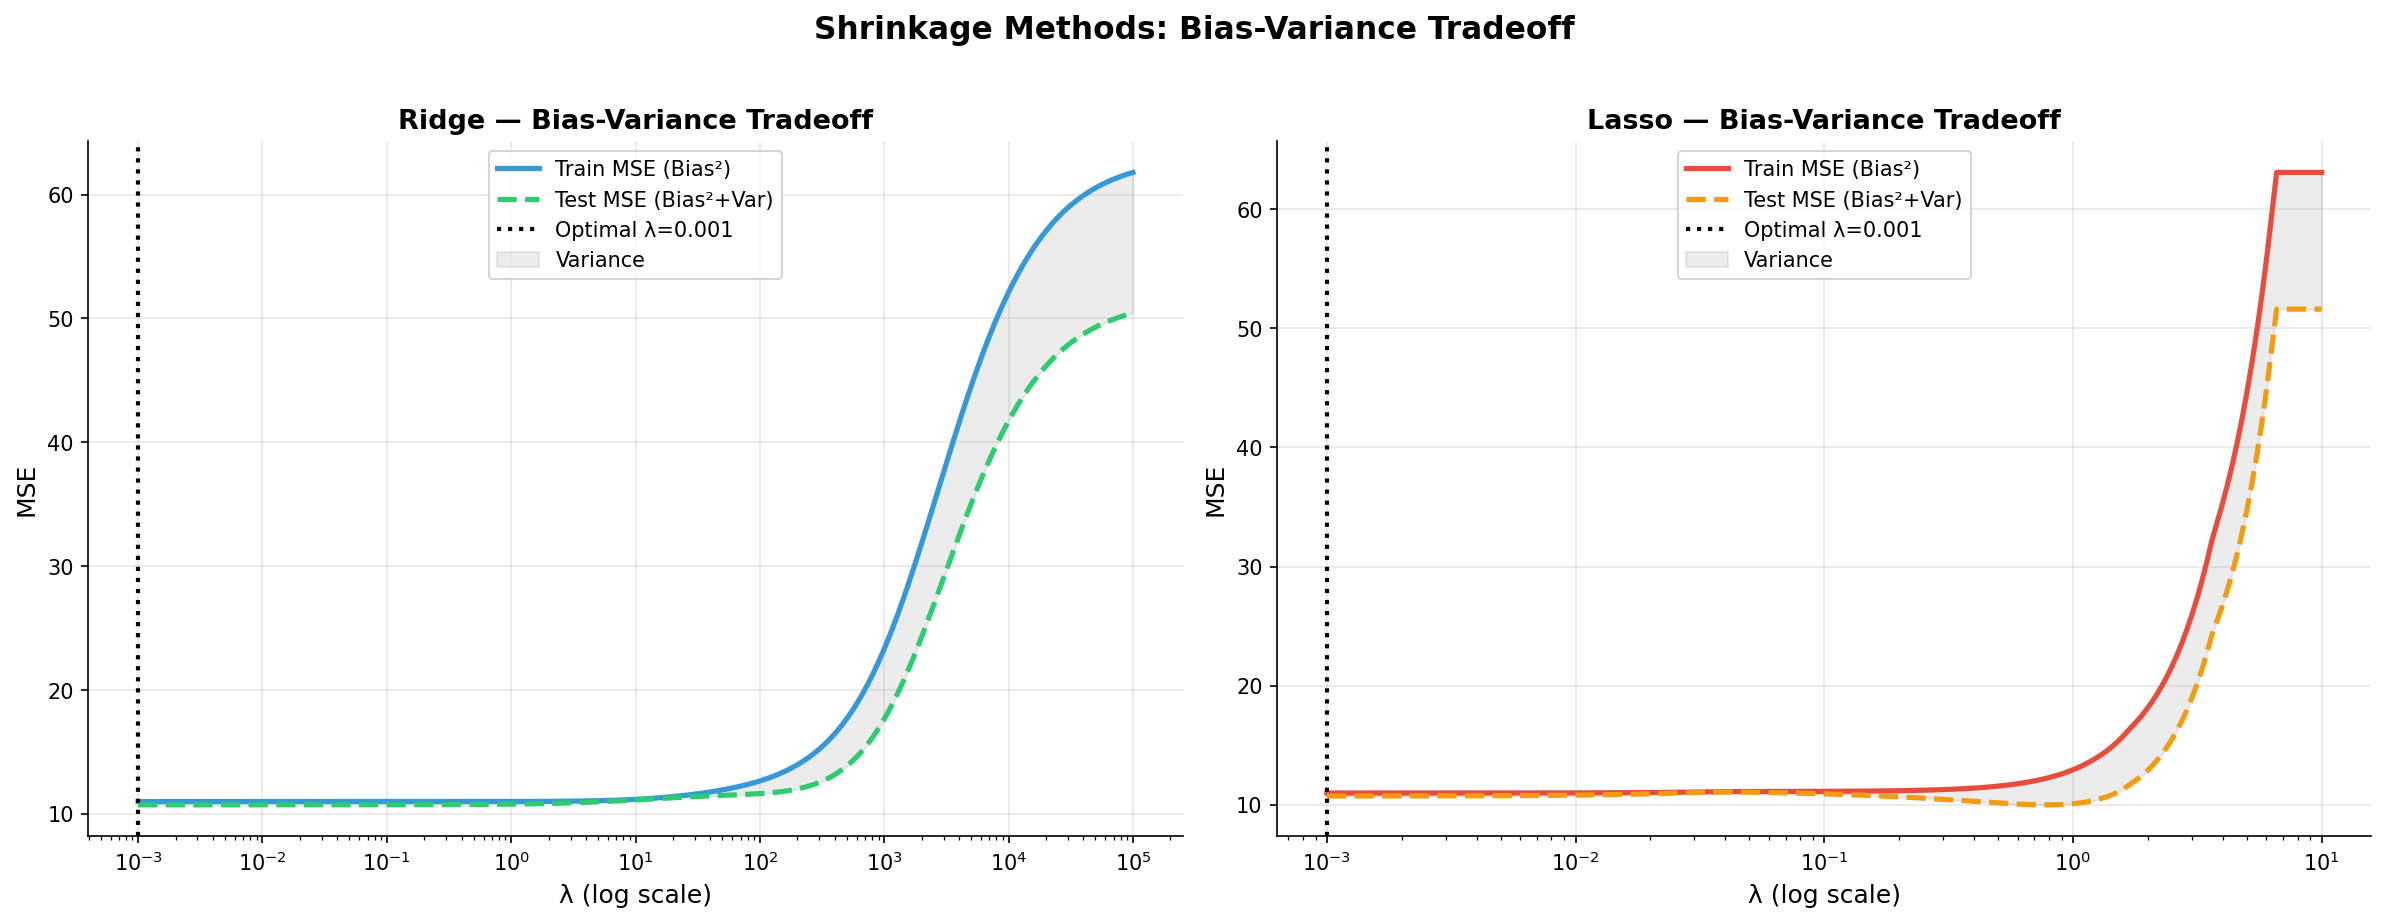
\includegraphics[width=\linewidth]{figures/bias_variance_tradeoff.png}
\caption{Bias--variance tradeoff for Ridge and Lasso: train MSE (solid) vs test MSE (dashed) vs $\lambda$. Optimal $\lambda$ minimizes test MSE.}
\label{fig:bias_var}
\end{figure}

\subsection{PCA and PLS}
\label{sec:pca_results}

PCA variance: PC1 explains 65.9\%, PC2 13.4\%, PC3 10.6\%. The first 3 components exceed 95\% cumulative variance. Table~\ref{tab:pcr_pls} shows PCR and PLS MSE vs number of components. PLS reaches OLS performance (MSE $\approx$ 11.45) with fewer components than PCR because PLS uses the target when constructing latent variables.

\begin{table}[htbp]
\caption{PCR and PLS: 10-fold CV MSE vs Number of Components}
\label{tab:pcr_pls}
\begin{center}
\begin{tabular}{|c|c|c|}
\hline
\textbf{Components} & \textbf{PCR MSE} & \textbf{PLS MSE} \\
\hline
1 & 16.99 & 15.73 \\
2 & 16.94 & 12.82 \\
3 & 13.25 & 12.11 \\
4 & 13.16 & 11.72 \\
5 & 12.65 & 11.63 \\
6 & 11.80 & 11.46 \\
7 & 11.45 & 11.45 \\
\hline
\end{tabular}
\end{center}
\end{table}

\begin{figure}[htbp]
\centering
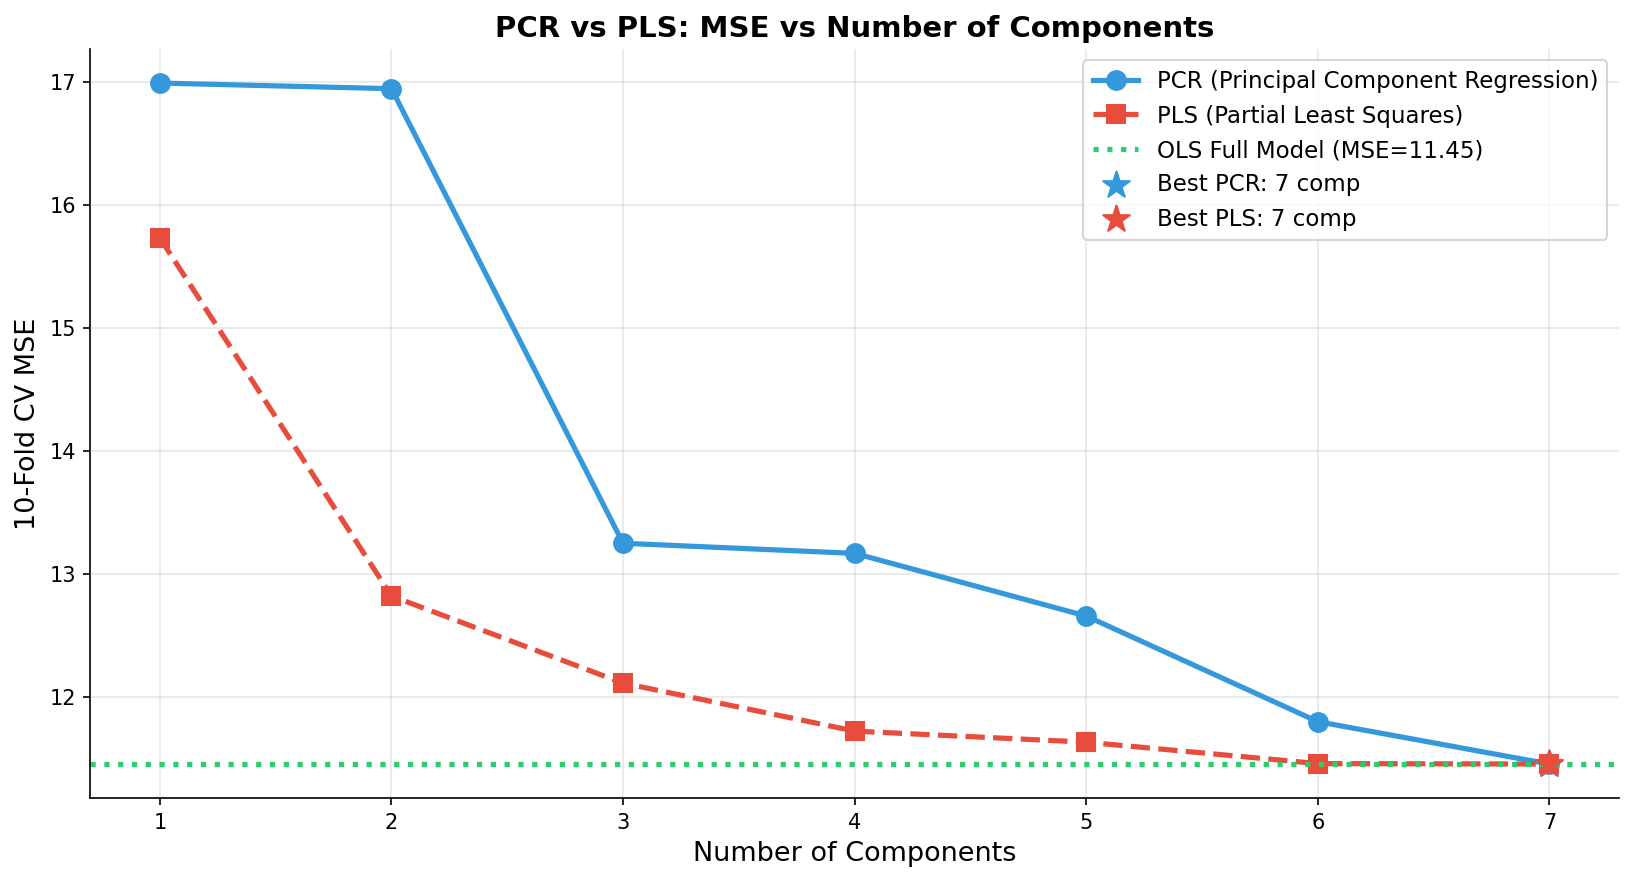
\includegraphics[width=\linewidth]{figures/pcr_pls_comparison.png}
\caption{PCR and PLS MSE vs number of components. PLS reaches OLS baseline with fewer components.}
\label{fig:pcr_pls}
\end{figure}

\subsection{Model Comparison}
\label{sec:comparison}

Table~\ref{tab:comparison} compares all six models. The \textbf{best model} is OLS with the optimal 4-feature subset: CV RMSE = 3.369, R$^2$ = 0.8113. Full OLS, Ridge, Lasso, PCR (7 comp), and PLS (7 comp) perform nearly identically (RMSE $\approx$ 3.384). The slight improvement from subset selection suggests that removing cylinders, horsepower, and acceleration reduces noise without losing predictive power.

\begin{table}[htbp]
\caption{Final Model Comparison (10-fold CV)}
\label{tab:comparison}
\begin{center}
\begin{tabular}{|l|c|c|c|}
\hline
\textbf{Model} & \textbf{CV MSE} & \textbf{CV RMSE} & \textbf{CV R$^2$} \\
\hline
OLS (all features) & 11.452 & 3.384 & 0.8085 \\
\textbf{OLS (best 4 subset)} & \textbf{11.353} & \textbf{3.369} & \textbf{0.8113} \\
Ridge ($\lambda = 0.001$) & 11.452 & 3.384 & 0.8085 \\
Lasso ($\lambda = 0.001$) & 11.451 & 3.384 & 0.8085 \\
PCR (7 comp) & 11.452 & 3.384 & 0.8085 \\
PLS (7 comp) & 11.452 & 3.384 & 0.8085 \\
\hline
\end{tabular}
\end{center}
\end{table}

\begin{figure}[htbp]
\centering
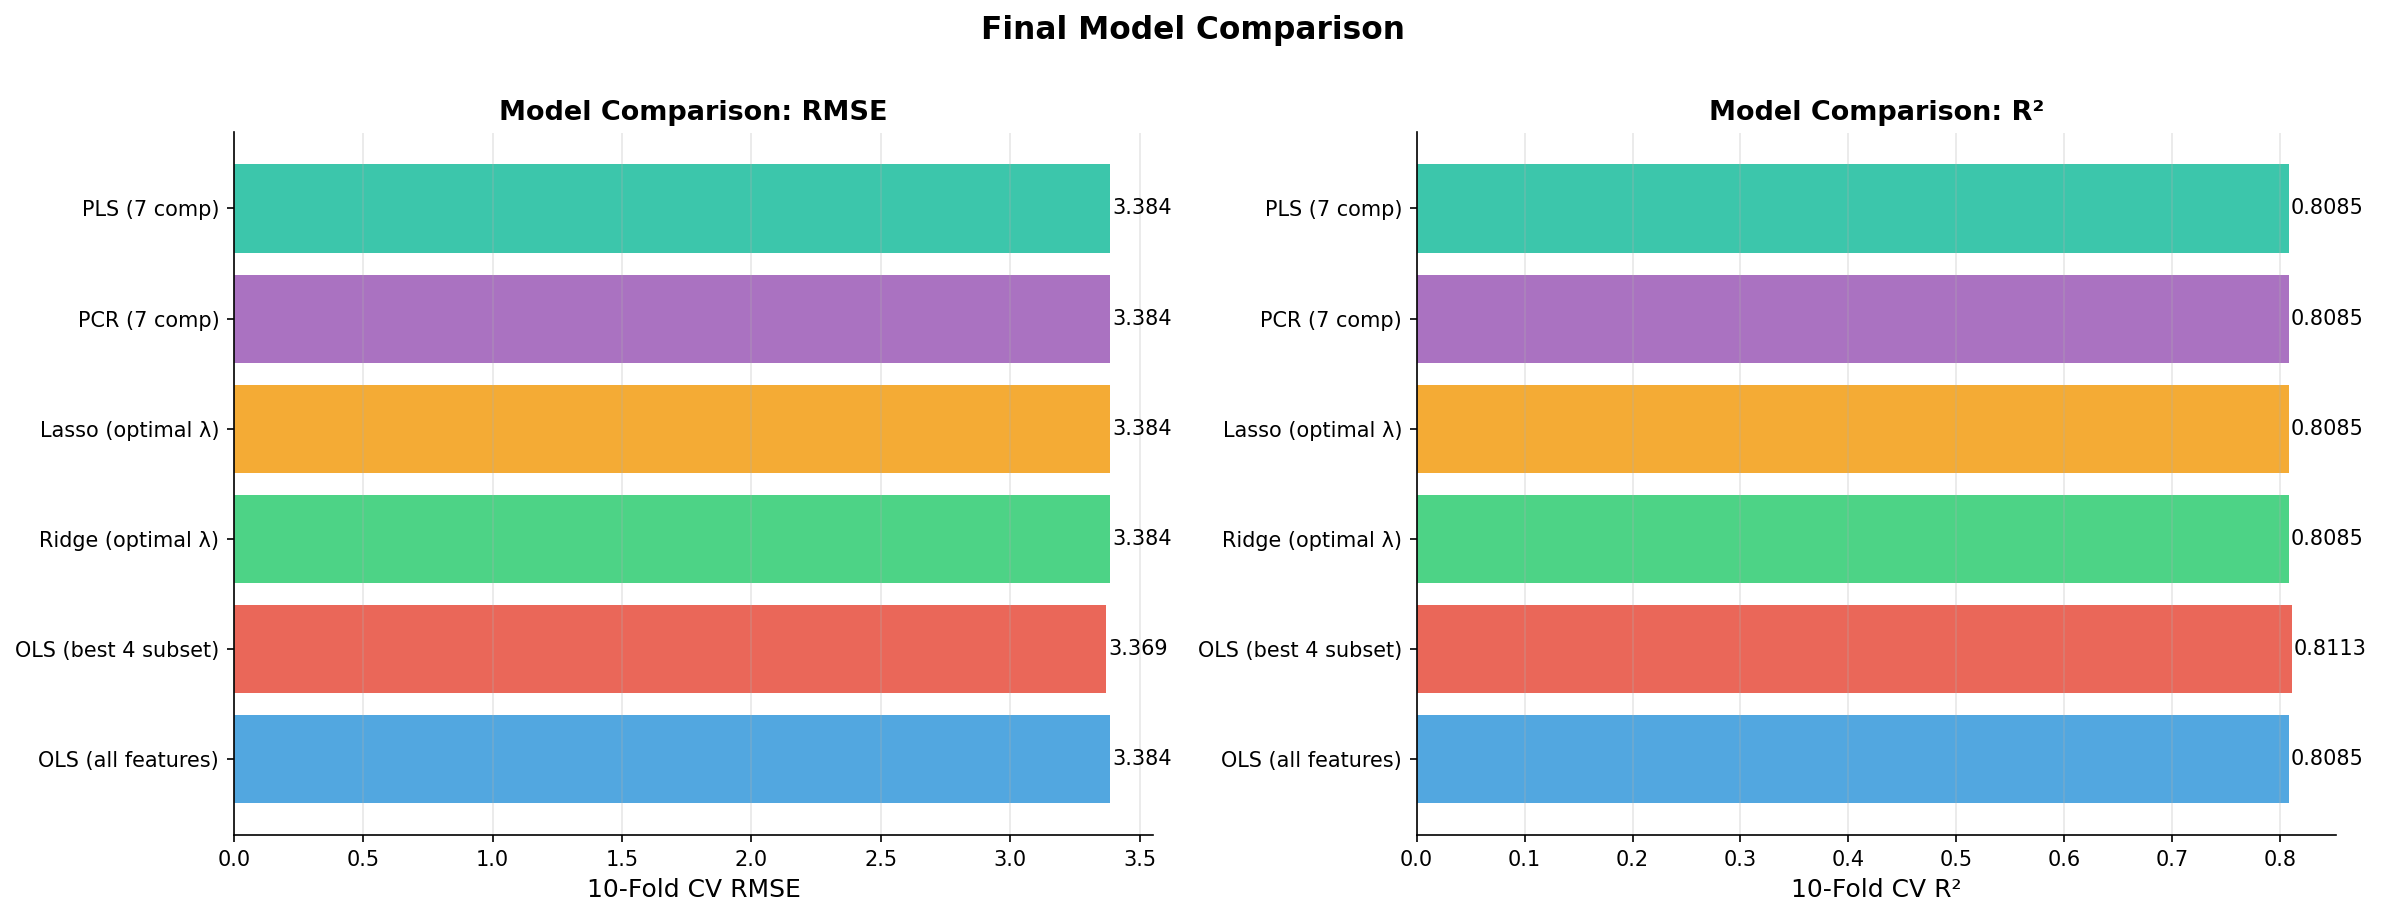
\includegraphics[width=\linewidth]{figures/model_comparison.png}
\caption{Final model comparison: CV RMSE and R$^2$ for all six models.}
\label{fig:comparison}
\end{figure}

\subsection{Interactive Dashboard}
An interactive Streamlit application demonstrates all methods and provides a Live Prediction Lab with car presets (e.g., 70s V8, 80s economy), algorithm selection, and feature contribution analysis. Run with \texttt{streamlit run streamlit\_app.py}. Source code and supplementary materials are available at \url{https://github.com/ggurbanov12098/AppliedML-P3}.

%==============================================================================
\section{Conclusion}
\label{sec:conclusion}
%==============================================================================

We applied resampling and model selection methods to the UCI Auto MPG dataset. Key findings:

\begin{itemize}
    \item \textbf{Resampling:} Degree 2 polynomial on weight is optimal for K=5, K=10, LOOCV, and bootstrap.
    \item \textbf{Subset selection:} Four predictors (displacement, weight, model\_year, origin) minimize CV MSE.
    \item \textbf{Shrinkage:} Ridge and Lasso both yield $\lambda = 0.001$; coefficients are nearly identical to OLS.
    \item \textbf{PCA/PLS:} PLS attains full performance with fewer components than PCR.
    \item \textbf{Best model:} OLS with the 4-feature subset (RMSE 3.369, R$^2$ 0.8113).
\end{itemize}

Future work could extend to non-linear models; larger datasets; and other feature engineering strategies.

%==============================================================================
\section*{Contributions}
\label{sec:contributions}
%==============================================================================

Riyad Abdurahimov and Gabil Gurbanov contributed jointly to this project. Both authors participated in data preprocessing, resampling implementation, subset selection, shrinkage methods (Ridge and Lasso), PCA/PLS analysis, model comparison, the Streamlit dashboard, report writing and presenting the project. The complete source code is available at \url{https://github.com/ggurbanov12098/AppliedML-P3}. Each team member is prepared to address questions related to the theoretical model and program code.

%==============================================================================
\section*{Abbreviations}
\label{sec:abbrev}
%==============================================================================

\vspace{0.5em}
\noindent
\small
\begin{tabular}{ll}
\textbf{AIC} & Akaike Information Criterion \\
\textbf{BIC} & Bayesian Information Criterion \\
\textbf{CV} & Cross-Validation \\
\textbf{LOOCV} & Leave-One-Out Cross-Validation \\
\textbf{MSE} & Mean Squared Error \\
\textbf{MPG} & Miles Per Gallon \\
\textbf{OOB} & Out-of-Bag \\
\textbf{OLS} & Ordinary Least Squares \\
\textbf{PCA} & Principal Component Analysis \\
\textbf{PCR} & Principal Component Regression \\
\textbf{PLS} & Partial Least Squares \\
\textbf{RMSE} & Root Mean Squared Error \\
\textbf{RSS} & Residual Sum of Squares \\
\textbf{UCI} & University of California, Irvine \\
\end{tabular}
\normalsize

%==============================================================================
% References
%==============================================================================

\begin{thebibliography}{00}
\sloppy

\bibitem{uci} D. Dua and C. Graff, ``UCI Machine Learning Repository,'' 2019. [Online]. Available: \url{https://archive.ics.uci.edu/ml/machine-learning-databases/auto-mpg/}

\bibitem{isl} G. James, D. Witten, T. Hastie, and R. Tibshirani, \textit{An Introduction to Statistical Learning with Applications in R}, 2nd~ed. Springer, 2021.

\bibitem{esl} T. Hastie, R. Tibshirani, and J. Friedman, \textit{The Elements of Statistical Learning}, 2nd~ed. Springer, 2009.

\bibitem{sklearn} F. Pedregosa et al., ``Scikit-learn: Machine Learning in Python,'' \textit{J. Mach. Learn. Res.}, vol.~12, pp.~2825--2830, 2011.

\bibitem{github} ``AppliedML-P3: Resampling and Model Selection on Auto MPG,'' GitHub repository. [Online]. Available: \url{https://github.com/ggurbanov12098/AppliedML-P3}

\end{thebibliography}

\end{document}
